\section{The commands}
\hypertarget{sec:com}{The} commands to achieve the Periodic Table of Elements are:
\begin{itemize}
\item\pgfPTMmacro{pgfPT}[]\ or \pgfPTMmacro{pgfPT}[options list] -- draws a full or partial graphical Periodic Table controlled by the optional keys.
\item\pgfPTMmacro{pgfPTstyle}[options list] -- sets the global style for the Periodic Table.
\item\pgfPTMmacro{pgfPTresetstyle}[] -- resets the style for the Periodic Table with the default values.
\item\pgfPTMmacro{pgfPTbuildcell}[]\blue{(}\textcolor{red!50!black}{nrows,ncolumns}\blue{)}\lp\red{entries}\rp%
\ -- builds the contents of each cell in the Periodic Table.
\item\pgfPTMmacro{pgfPTresetcell}[] -- resets the cell to its default layout.%
\item\pgfPTMmacro{pgfPTbuildcellstyle}[]\lb\red{name}\rb\blue{(}\red{nrows,ncolumns}\blue{)}\lp\red{entries}\rp%
\ -- builds the contents of each cell in the Periodic Table and stores it in a named style.
%\item\pgfPTMmacro{showcellinfo}[] -- shows the information about the contents of the last unnamed builded cell. If no cells have yet been build, the default cell is shown.
%\item\pgfPTMmacro{showcellstyleinfo}[]\textcolor{blue!50!black}{(}\textcolor{red!50!black}{name}\textcolor{blue!50!black}{)} -- shows the information about the contents of the named builded cell.
\item\pgfPTMmacro{pgfPTpreviewcell}[]\ or \pgfPTMmacro{pgfPTpreviewcell}[scale factor] -- preview the last unnamed built cell with an optional scale factor. If no cells have yet been built, the default cell is shown.
\item\pgfPTMmacro{pgfPTpreviewcellstyle}[]\lb\red{name}\rb%
\ or \pgfPTMmacro{pgfPTpreviewcellstyle}[]\lp\red{scale factor}\rp\lb\red{name}\rb%
\ -- preview the named builded cell with an optional scale factor.
\item\pgfPTMmacro{pgfPTnewcolorscheme}[trailing color]\lb\red{name}\rb\lb\red{color list}\rb%
\ -- makes a color scheme to fill the cells along the Periodic Table.
\item\pgfPTMmacro{pgfPTnewZlist}[]\lb\red{name}\rb%
\ -- create a user defined atomic numbers (Z) \red{named} list.
\item\pgfPTMmacro{pgfPTsetLanguage}[]\lb\red{language flag}\rb%
\ -- globally change the default language.
\end{itemize}
\vspace{-32pt}\ %
\def\tmpSection{\bs{pgfPT}}%
\subsection*{}{\normalfont\large\bfseries\raisebox{1.25pt}{$\mathbf{\blacktriangleright}$}\ Utilization of \tmpSection}%
\label{command:pgfPT}\addcontentsline{toc}{subsection}{\texorpdfstring{\tmpSection{}}{\textbackslash pgfPT}}%
\index{COMMANDS@\textbf{COMMANDS}!\textbackslash pgfPT}%
\\ [4pt]Use this command to draw the Periodic Table of Elements in the language selected at package inclusion (\texttt{\large\textcolor{green!40!black}{\textbackslash usepackage}\textcolor{blue!70!black}{[}\textcolor{brown!60!black}{language flag}\textcolor{blue!70!black}{]}\textcolor{purple!70!black}{\{}\textcolor{blue!70!black}{pgf-PeriodicTable}\textcolor{purple!40!black}{\}}}):
\\ [5pt]\pgfPTMmacrobox{pgfPT}[]%
\\ [10pt]\makebox[\linewidth][c]{\scalebox{.6}{\pgfPT}}%
\\ [0pt]\pgfPTMline%
\newpage%
This command can also be used with options -- as described in section \hyperlink{OPTIONS}{Options for \textbackslash pgfPT: creating a �Periodic Table�} -- to modify, for instance, the font of the Periodic Table or the colors of the cells:
\\ [10pt]\pgfPTMmacrobox{pgfPT}[font=pnc,back color scheme=MNM]%
\\ [10pt]\makebox[\linewidth][c]{\scalebox{.6}{\pgfPT[font=pnc,back color scheme=MNM]}}%
\\ [0pt]\pgfPTMline%
%%%%%%%%%%%%%%%%%%%%%%%%%%%%%%%%%%%%%%%%%%%%%%%%%%%%%%%%%%%%
\\ [-32pt]\ %
\def\tmpSection{\bs{pgfPTstyle}\lp\red{options list}\rp}%
\subsection*{}{\normalfont\large\bfseries\raisebox{1.25pt}{$\mathbf{\blacktriangleright}$}\ Utilization of \tmpSection}%
\label{command:pgfPTstyle}\addcontentsline{toc}{subsection}{\texorpdfstring{\tmpSection{}}{\textbackslash pgfPTstyle}}%
\index{COMMANDS@\textbf{COMMANDS}!\textbackslash pgfPTstyle}%
\\ [4pt]This command globally sets a style for the Periodic Table:
\\ [10pt]\pgfPTMmacrobox[l]{pgfPTstyle}[font=ptm,IUPAC=false,show title=false]%
\pgfPTstyle[font=ptm,IUPAC=false,show title=false]%
\\ [-4pt]\pgfPTMmacrobox{pgfPT}[]%
\\ [10pt]\makebox[\linewidth][c]{\scalebox{.6}{\pgfPT}}%
\\ [0pt]\pgfPTMline%
\newpage%\\ [5pt]
It is possible to locally override the \textit{global style} defined:
\\ [5pt]\pgfPTMmacrobox{pgfPT}[show title]%
\\ [10pt]\makebox[\linewidth][c]{\scalebox{.6}{\pgfPT[show title]}}%
\\ [5pt]\pgfPTMline%
%%%%%%%%%%%%%%%%%%%%%%%%%%%%%%%%%%%%%%%%%%%%%%%%%%%%%%%%%%%%
%\newpage\ \\ [-62pt]%
\\ [-32pt]\ %
\def\tmpSection{\bs{pgfPTresetstyle}}%
\subsection*{}{\normalfont\large\bfseries\raisebox{1.25pt}{$\mathbf{\blacktriangleright}$}\ Utilization of \tmpSection}%
\label{command:pgfPTresetstyle}\addcontentsline{toc}{subsection}{\texorpdfstring{\tmpSection{}}{\textbackslash pgfPTresetstyle}}%
\index{COMMANDS@\textbf{COMMANDS}!\textbackslash pgfPTresetstyle}%
\\ [4pt]This command resets the style used in the Periodic Table to default values:
\\ [10pt]\pgfPTMmacrobox[l]{pgfPTresetstyle}[]%
\pgfPTresetstyle%
\\ [-4pt]\pgfPTMmacrobox{pgfPT}[]%
\\ [10pt]\makebox[\linewidth][c]{\scalebox{.6}{\pgfPT}}%
\\ [0pt]\pgfPTMline%
%%%%%%%%%%%%%%%%%%%%%%%%%%%%%%%%%%%%%%%%%%%%%%%%%%%%%%%%%%%%
\newpage\ \\ [-62pt]
%\\ [-32pt]\ %
\def\tmpSection{\bs{pgfPTbuildcell}\blue{(}\red{nrows,ncolumns}\blue{)}\lp\red{entries}\rp}%
\subsection*{}{\color{black}\normalfont\large\bfseries\raisebox{1.25pt}{$\mathbf{\blacktriangleright}$}\ Utilization of \tmpSection}%
\label{command:pgfPTbuildcell}\addcontentsline{toc}{subsection}{\texorpdfstring{\tmpSection{}}{\textbackslash pgfPTbuildcell}}%
\index{COMMANDS@\textbf{COMMANDS}!\textbackslash pgfPTbuildcell}%
\\ [4pt]With \pgfPTMmacro{pgfPTbuildcell}[] it is possible to customize the \textit{elementar} cell of the Periodic Table. Each cell is built on the given \textit{number of rows} and \textit{number of columns}. After that, each \textit{entry} is constructed according to the structure \red{row;column;what} or \red{initial row-final row;initial column-final column;what}.
\vspace{8pt}%
\begin{itemlist}
\item The first \textit{syntax} -- \red{row;column;what} -- puts �\red{what}� in the �\red{row}� row and in the �\red{column}� column with the height of one row and the width of one column:
\\ -- for example, \red{1;1;Z} puts the atomic number \red{Z} in row \red{1} and column \red{1}, witch actually corresponds to a box anchored to the top left corner of the cell and that \textit{goes} below and to the right of that corner.
\item The second \textit{syntax} -- \mbox{\red{initial row-final row;initial column-final column;what}} -- puts �\red{what}� from �\red{initial row}� to �\red{final row}� with the height of $\textsf{\large final row}-\textsf{\large initial row}+\textsf{1}$ and from �\red{initial column}� to �\red{final column}� with the width of $\textsf{\large final column}-\textsf{\large initial column}+\textsf{1}$. It is important to keep in mind that when using this syntax the \textit{row} and \textit{column} could have any value between \textbf{1} and \textbf{number of rows} and \textbf{number of columns}, respectively.
\\ -- for example, \red{1;1-2.1;Z} puts the atomic number \red{Z} in row \red{1} with the height of one row and from column \red{1} to \textit{column} \red{2\mbox{.}1}, with the width of $\textsf{2\mbox{.}1}\times\textsf{\large column}$. Note that in this example the two \textit{syntaxes} are mixed up.
\end{itemlist}
\vspace{8pt}The \textbf{default cell} of the Periodic Table is constructed with the command:
\\ [10pt]\pgfPTMbuildcell(5,3)[(1;1-2;Z),(1;3;radio),(2-3;1.5-2.5;CS),(4;1-3;name),(5;1-3;Ar)]
%%%%%%%%%%%%%%%%%%%%%%%%%%%%%%%%%%%%%%%%%%%%%%%%%%%%%%%%%%%%
\\ [-32pt]\ %
\def\tmpSection{\bs{pgfPTresetcell}}%
\subsection*{}{\normalfont\large\bfseries\raisebox{1.25pt}{\color{black}$\mathbf{\blacktriangleright}$}\ Utilization of \tmpSection}%
\label{command:pgfPTresetcell}\addcontentsline{toc}{subsection}{\texorpdfstring{\tmpSection{}}{\textbackslash pgfPTbuildcellstyle}}%
\index{COMMANDS@\textbf{COMMANDS}!\textbackslash pgfPTresetcell}%
\\ [4pt]The \pgfPTMmacro{pgfPTresetcell}[] resets the cell to its default layout.
\\ [-32pt]\ %
\def\tmpSection{\bs{pgfPTbuildcellstyle}\lb\red{name}\rb\blue{(}\red{nrows,ncol...}\blue{)}\lp\red{entr...}\rp}%
\def\tmpSectionTOC{\bs{pgfPTbuildcellstyle}\lb\red{name}\rb\blue{(}\red{nrows,ncolumns}\blue{)}\lp\red{entries}\rp}%
\subsection*{}{\normalfont\large\bfseries\raisebox{1.25pt}{\color{black}$\mathbf{\blacktriangleright}$}\ Utilization of \tmpSection}%
\label{command:pgfPTbuildcellstyle}\addcontentsline{toc}{subsection}{\texorpdfstring{\tmpSectionTOC{}}{\textbackslash pgfPTbuildcellstyle}}%
\index{COMMANDS@\textbf{COMMANDS}!\textbackslash pgfPTbuildcellstyle}%
\\ [4pt]The \pgfPTMmacro{pgfPTbuildcellstyle}[] command works like \pgfPTMmacro{pgfPTbuildcell}[], but stores the cell style under the \textcolor{red!50!black}{name} provided. It is only used when called via the \textcolor{red!50!black}{cell style} passed as an option to \pgfPTMmacro{pgfPT}[]. Otherwise it remains unavailable, unlike the \pgfPTMmacro{pgfPTbuildcell}[] command which immediately affects the cells of the Periodic Table.
%%%%%%%%%%%%%%%%%%%%%%%%%%%%%%%%%%%%%%%%%%%%%%%%%%%%%%%%%%%%
\\ [-32pt]\ %
\def\tmpSection{\bs{pgfPTpreviewcell}}%
\subsection*{}{\normalfont\large\bfseries\raisebox{1.25pt}{$\mathbf{\blacktriangleright}$}\ Utilization of \tmpSection}%
\label{command:pgfPTpreviewcell}\addcontentsline{toc}{subsection}{\texorpdfstring{\tmpSection{}}{\textbackslash pgfPTpreviewcell}}%
\index{COMMANDS@\textbf{COMMANDS}!\textbackslash pgfPTpreviewcell}%
\\ [4pt]The main purpose of this command is to show the built cell for \textit{debugging}.
\\ With \pgfPTMmacro{pgfPTpreviewcell}[] you can preview the last unnamed built cell with an optional \red{scale factor}. If no cells have yet been built, the default cell is shown.
\\ [5pt]\pgfPTMmacrobox{pgfPTpreviewcell}[]%
\\ [10pt]\pgfPTpreviewcell%
\\ [5pt]\pgfPTMline%
\\ [10pt]\pgfPTMbuildcell(8,3)[(1;1-2;Z),(1;3;radio),(2-3;1.5-3.5;CS),(4-5;1-3;name), %
(6;1-3;spectra),(7;1-3;DiscC),(8;1-3;DiscY)]%
\pgfPTbuildcell(8,3)[(1;1-2;Z),(1;3;radio),(2-3;1.5-3.5;CS),(4-5;1-3;name),%
(6;1-3;spectra),(7;1-3;DiscC),(8;1-3;DiscY)]%
\\ [-4pt]\pgfPTMmacrobox{pgfPTpreviewcell}[1.8]%
\\ [10pt]\pgfPTpreviewcell[1.8]%
\\ [5pt]\pgfPTMline%
%%%%%%%%%%%%%%%%%%%%%%%%%%%%%%%%%%%%%%%%%%%%%%%%%%%%%%%%%%%%
\\ [-32pt]\ %
\def\tmpSection{\bs{pgfPTpreviewcellstyle}\lb\red{name}\rb}%
\subsection*{}{\normalfont\large\bfseries\raisebox{1.25pt}{$\mathbf{\blacktriangleright}$}\ Utilization of \tmpSection}%
\label{command:pgfPTpreviewcellstyle}\addcontentsline{toc}{subsection}{\texorpdfstring{\tmpSection{}}{\textbackslash pgfPTpreviewcellstyle}}%
\index{COMMANDS@\textbf{COMMANDS}!\textbackslash pgfPTpreviewcellstyle}%
\\ [4pt]This previews a \textit{named} cell, again with the optional \red{scale factor}.
\\ [5pt]\pgfPTMpreviewcellstyle[]{myname}%
\\ [10pt]\pgfPTpreviewcellstyle{myname}%
\\ [5pt]\pgfPTMline%
\\ [10pt]\pgfPTMbuildcellstyle{myname}(5,3)[(1;1-2;Z),(1;3;radio),(2-3;1.5-3.5;CS),(4;1-3;name),(5;1-3;Ar*)]%
\pgfPTbuildcellstyle{myname}(5,3)[(1;1-2;Z),(1;3;radio),(2-3;1.5-3.5;CS),(4;1-3;name),(5;1-3;Ar*)]%
\\ [-4pt]\pgfPTMpreviewcellstyle[2]{myname}%
\\ [10pt]\pgfPTpreviewcellstyle[2]{myname}%
\\ [5pt]\pgfPTMline%
%%%%%%%%%%%%%%%%%%%%%%%%%%%%%%%%%%%%%%%%%%%%%%%%%%%%%%%%%%%%
\\ [-32pt]\ %
\def\tmpSection{\bs{pgfPTnewColorScheme}\lb\red{name}\rb\lp\red{color list}\rp}%
\subsection*{}{\normalfont\large\bfseries\raisebox{1.25pt}{$\mathbf{\blacktriangleright}$}\ Utilization of \tmpSection}%
\label{command:pgfPTnewColorScheme}\addcontentsline{toc}{subsection}{\texorpdfstring{\tmpSection{}}{\textbackslash pgfPTnewColorScheme}}%
\index{COMMANDS@\textbf{COMMANDS}!\textbackslash pgfPTnewColorScheme}%
\\ [4pt]Use this command to create a \textit{color scheme} for cells in the Periodic Table. It has two mandatory arguments -- \red{name} and \red{color list} -- and an optional argument -- \red{trailing color}.
\\ [4pt]The \red{name} is used to identify the \textit{color scheme}. The \red{color list} is a comma-separated list of red, green and blue values written as r/g/b, defined in ascending order of Z and starting at Z=1. The optional argument \red{trailing color} is appended to the end of the list and is used for all cells starting from this point on. It also has the form r/g/b and its default value is 1/1/1 (white).
\\ [10pt]\pgfPTMnewColorScheme[]{myname}{.5/.5/.5,1/0/0,0/1/0,0/0/1}%
\pgfPTnewColorScheme{myname}{.5/.5/.5,1/0/0,0/1/0,0/0/1}%
\\ [-4pt]\pgfPTMmacrobox{pgfPT}[back color scheme=myname]%
\\ [10pt]\makebox[\linewidth][c]{\scalebox{.6}{\pgfPT[back color scheme=myname]}}%
\\ [0pt]\pgfPTMline%
\\ [10pt]\pgfPTMnewColorScheme[.25/.25/.25]{myname}{.5/.5/.5,1/0/0,0/1/0,0/0/1}%
\pgfPTnewColorScheme[.25/.25/.25]{myname}{.5/.5/.5,1/0/0,0/1/0,0/0/1}%
\\ [-4pt]\pgfPTMmacrobox{pgfPTresetcell}[]%
\pgfPTresetcell%
\\ [-4pt]\pgfPTMmacrobox{pgfPT}[back color scheme=myname,name color=white, Ar color=white,legend back color=black!30]%
\\ [10pt]\makebox[\linewidth][c]{\scalebox{.6}{\pgfPT[back color scheme=myname,name color=white,Ar color=white,legend back color=black!30]}}%
\\ [0pt]\pgfPTMline%
\newpage%\\ [10pt]
There are a few \textit{color schemes} predefined:
\index{BUILT-IN@\textbf{BUILT-IN}!color schemes}%
\begin{itembar}
\item\textbf{default}, the default built-in color scheme, which is loaded if no value is passed to the \red{back color scheme} key.
\item\textbf{Soft}, a soft color pattern for cells, differentiating metals, non metals, semimetals, lanthanides and actinides.
\item\textbf{Jmol}, a color scheme based upon \href{http://www.jmol.org/}{Jmol: an open-source Java viewer for chemical structures in 3D}.
\item\textbf{CPK}, a color scheme that is based upon the colors of the popular plastic spacefilling models which were developed by Corey, Pauling and later improved by Kultun.
\item\textbf{Rasmol} and \textbf{RasmolNew}, two color schemes based upon the computer program \href{http://www.rasmol.org/}{RasMol}.
\item\textbf{Wikipedia}, a color scheme built on the Periodic Table of Elements available at \href{https://en.wikipedia.org/wiki/Periodic_table#Classification_of_elements}{Wikipedia}.
\item\textbf{MNM}, a color pattern which distinguishes between \textbf{M}etals, semimetals and \textbf{N}on \textbf{M}etals.
\item\textbf{PS}, a color scheme depicting the \textbf{P}hysical \textbf{S}tate at room temperature.
\item\textbf{Radio}, a two color color scheme showing the radioactivity of the elements.
\item\textbf{Blocks}, a four colored color scheme showing the \textit{s}, \textit{p}, \textit{d} and \textit{f} blocks of the Periodic Table.
\end{itembar}
\vspace{5pt}
Writing a color scheme can be painstaking work, so a \textit{script} is provided for that:
\\ [5pt]\makebox[\linewidth][c]{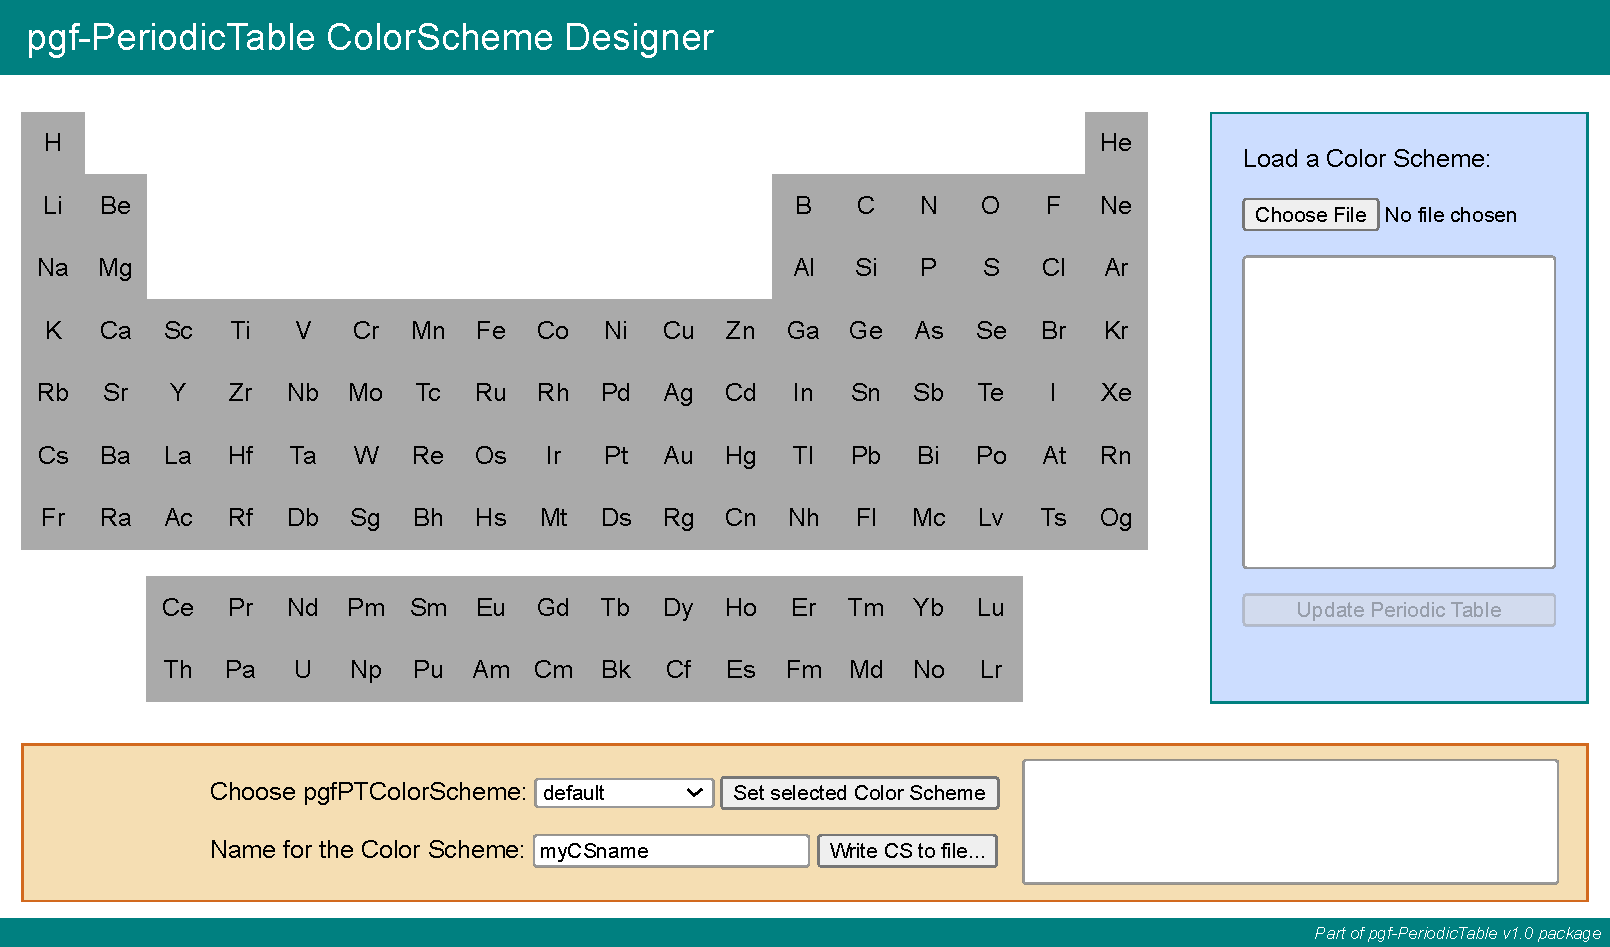
\includegraphics[height=5.2cm]{manualfiles/pgfPTcolorSchemes_html_general.pdf}}
\\ [5pt]\makebox[\linewidth][c]{\href{run:pgfPTcolorSchemes.html}{pgfPTcolorSchemes.html}}
%%%%%%%%%%%%%%%%%%%%%%%%%%%%%%%%%%%%%%%%%%%%%%%%%%%%%%%%%%%%
%\newpage\ \\ [-62pt]
\\ [-32pt]\ %
\def\tmpSection{\bs{pgfPTnewZlist}\lb\red{name}\rb}%
\subsection*{}{\normalfont\large\bfseries\raisebox{1.25pt}{$\mathbf{\blacktriangleright}$}\ Utilization of \tmpSection}%
\index{COMMANDS@\textbf{COMMANDS}!\textbackslash pgfPTnewZlist}%
\label{command:pgfPTnewZlist}\addcontentsline{toc}{subsection}{\texorpdfstring{\tmpSection{}}{\textbackslash pgfPTnewZlist}}%
\\ [4pt]This command makes a user defined atomic numbers' list with the provided \textcolor{red!50!black}{name}. The list can be anything that the {\large\textsf{\textbackslash foreach}} loop, defined in the \txttikz{} package, can understand.
\\ [2pt]{\small For more information on how to use {\normalsize\textsf{\textbackslash foreach}} loop refer to the section \textit{Repeating Things: The Foreach Statement} in the \href{https://www.ctan.org/pkg/pgf}{pgfmanual}}.
\\ [10pt]\pgfPTMnewZlist{myZlist}{1,...,57,72,80,81,...,85}%
\pgfPTnewZlist{myZlist}{1,...,57,72,80,81,...,85}%
\\ [-4pt]\pgfPTMmacrobox{pgfPT}[Z list=myZlist,IUPAC=false]%
\\ [10pt]\makebox[\linewidth][c]{\scalebox{.6}{\pgfPT[Z list=myZlist,IUPAC=false]}}%
\\ [5pt]\pgfPTMline%
\newpage\ \\ [-62pt]
%\\ [-32pt]\ %
\def\tmpSection{\bs{pgfPTsetLanguage}\lb\red{language flag}\rb}%
\subsection*{}{\normalfont\large\bfseries\raisebox{1.25pt}{$\mathbf{\blacktriangleright}$}\ Utilization of \tmpSection}%
\index{COMMANDS@\textbf{COMMANDS}!\textbackslash pgfPTsetLanguage}%
\label{command:pgfPTsetLanguage}\addcontentsline{toc}{subsection}{\texorpdfstring{\tmpSection{}}{\textbackslash pgfPTsetLanguage}}%
\\ [4pt]This command globally changes the default language of the Periodic Table.
\\ [10pt]\pgfPTMsetLanguage{pt}%
\pgfPTsetLanguage{pt}%
\\ [-4pt]\pgfPTMmacrobox{pgfPT}[]%
\\ [10pt]\makebox[\linewidth][c]{\scalebox{.6}{\pgfPT[]}}%
\\ [10pt]\pgfPTMsetLanguage{en}%
\pgfPTsetLanguage{en}%
\\ [-4pt]\pgfPTMmacrobox{pgfPT}[]%
\\ [10pt]\makebox[\linewidth][c]{\scalebox{.6}{\pgfPT[]}}%
\\ [5pt]\pgfPTMline%
\endinput
